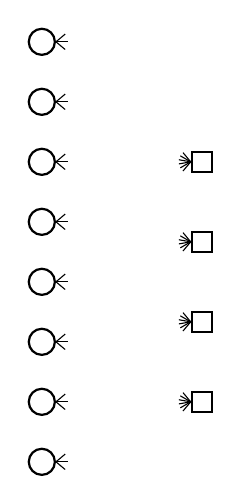
\begin{tikzpicture}
\def\horzgap{0.8in}; %Horizontal gap between nodes/levels
\def \gapVN{0.3in}; %vertical gap between nodes
\def \gapCN{0.4in}; %Horizontal gap between nodes

\def \textoffs{0.12in}; %Offset for writing text above a node
\def\nodewidth{0.1in};
\def\ext{0.06in};



\def \n {8};
\def\ldeg{3};
\def \m {4};
\def\rdeg{6};
\def\langle{40};%120 degrees/3
\def\langle{20};%120 degrees/6

\tikzstyle{check} = [rectangle, draw, text centered, thick, 
                          minimum height=\nodewidth, minimum width=\nodewidth]
\tikzstyle{bit} = [circle, draw, text centered, thick,
                          radius=0.5*\nodewidth]
                          
\foreach \vn in {1,...,\n}{
 \node[bit] (vn\vn) at (0,\vn*\gapVN) {};
 \draw (vn\vn.east) --+ (+40:\ext); 
  \draw (vn\vn.east) --+ (0:\ext); 
   \draw (vn\vn.east) --+ (-40:\ext); 
}


\foreach \cn in {1,...,\m}{
\node[check] (cn\cn) at (\horzgap,0.2in+\cn*\gapCN) {};

 \draw (cn\cn.west) --+ (+130:\ext); 
 \draw (cn\cn.west) --+ (+150:\ext); 
 \draw (cn\cn.west) --+ (+170:\ext); 
 \draw (cn\cn.west) --+ (+190:\ext); 
 \draw (cn\cn.west) --+ (+210:\ext); 
 \draw (cn\cn.west) --+ (+230:\ext); 
}

\end{tikzpicture}